%-------------------------------------------------------------------------------
\chapter{Modeling of a humanoid robot}
\label{ch.modeling}
\acresetall
%-------------------------------------------------------------------------------

A very abstract model of a humanoid robot~\cref{eq.general_system} was
sufficient for the discussion in \cref{ch.balance}, but it is of no use for
practical applications. Therefore, in the present chapter we specify and study
the structure of humanoid robot models. Though we employ only the whole body
model for control (\cref{sec.whole_body_model}) and approximate linear models
for anticipation (\cref{sec.linear_approx_models}), we also consider
approximate nonlinear models in \cref{sec.nonlinear_approx_models} to
demonstrate the ancestral relationships between these models. These
relationships can be illustrated with the following tree

\begin{forest}
  for tree={
    grow'=0,
    child anchor=west,
    parent anchor=south,
    anchor=west,
    calign=first,
    edge path={
      \noexpand\path [draw, \forestoption{edge}]
      (!u.south west) +(7.5pt,0) |- node[fill,inner sep=1.25pt] {} (.child anchor)\forestoption{edge label};
    },
    before typesetting nodes={
      if n=1
        {insert before={[,phantom]}}
        {}
    },
    fit=band,
    before computing xy={l=25pt},
  }
[Whole body (\nameref{model.WB}) model (\cref{sec.whole_body_model})
    [Nonlinear momenta-based (\nameref{model.NMB}) model (\cref{sec.momenta_based_nonlinear})
        [Nonlinear point-mass (\nameref{model.NPM}) model (\cref{sec.point_mass_nonlinear})
            [\begin{minipage}{11cm}Linear point-mass models (\nameref{model.CPPMJ} and \nameref{model.CPPMdZ}) with planar \ac{CoM} motion (\cref{sec.point_mass_planar})\end{minipage}]
            [\begin{minipage}{11cm}Linear point-mass model (\nameref{model.CNPM}) with nonplanar \ac{CoM} motion (\cref{sec.point_mass_nonplanar})\end{minipage}]
        ]
    [Linear momenta-based (\nameref{model.CMB}) model (\cref{sec.model_momenta})]
  ]
]
\end{forest}


We present detailed derivations of the models and try to be explicit about all
assumptions made in the process. Most of the assumptions are introduced to
linearize models in order to fit them in the \ac{PLLS} framework
(\cref{ch.optimization}), which we employ for both control and anticipation.



%%%%%%%%%%%%%%%%%%%%%%%%%%%%%%%%%%%%%%%%%%%%%%%%%%%%%%%%%%%%%%%%%%%%%%%%%%%%%%%%
%%%%%%%%%%%%%%%%%%%%%%%%%%%%%%%%%%%%%%%%%%%%%%%%%%%%%%%%%%%%%%%%%%%%%%%%%%%%%%%%
%%%%%%%%%%%%%%%%%%%%%%%%%%%%%%%%%%%%%%%%%%%%%%%%%%%%%%%%%%%%%%%%%%%%%%%%%%%%%%%%
\section{Whole body dynamical model}\label{sec.whole_body_model}

We start by considering the whole body model of a humanoid robot. A humanoid
robot is a chain of $n+1$ links interconnected by $n$ joints. In general,
joints can be rotary or prismatic, actuated or not actuated. While all these
joint types can be incorporated in the model without much effort, we limit our
discussion to actuated rotary joints only, since the other types are rare in
humanoid robots. The links composing the robot can be in contact with the
environment, but are not fixed to any support. Therefore, the robot must be
modeled taking contacts and contact friction into account. We use \tn{Coulomb's
law} as a friction model \cite[Chapter~10]{Popov2010contact} and make the
following additional assumptions:
%
\begin{description}
    \item[\ass{ass.frictioncoef}] coefficients of static and kinetic (dynamic)
        friction are equal and constant \cite[Chapter~10]{Popov2010contact};
    \item[\ass{ass.norolling}] there are no rolling contacts;
    \item[\ass{ass.rigid}] the environment and links of the robot are rigid;
    \item[\ass{ass.fixed_environment}] the robot contacts only the objects,
        whose positions are fixed in the environment;
    \item[\ass{ass.nojointfriction}] there is no friction in the joints;
    \item[\ass{ass.nouncertainty}] there are no noises in measurements of the
        state and no inaccuracies in parameters of the robot.
\end{description}
%
\cref{ass.frictioncoef} is ubiquitous in the literature.
\cref{ass.norolling,ass.rigid,ass.fixed_environment} are not valid in some
settings, but we do not consider such settings and thus avoid the burden of
more accurate modeling. The last two assumptions can never be fulfilled in
practice. However, friction in the joints can be modeled, if the corresponding
parameters of the robot are provided, or it can be concealed by joint-level
position controllers of a robot such as \sn{HRP-2} \cite{Kaneko2004icra}. The
problem of uncertainty, on the other hand, is not addressed by modeling, but
rather by robust control and techniques for estimation of parameters and state
\cite[Chapter~8]{Siciliano2010robotics}, \cite{Christensen2008handbook}. We
leave such topics outside of the scope of this thesis.


Based on the listed assumptions, we present the whole body model in the
following \cref{sec.complementarity_system}.
\cref{sec.wbm_constraints,sec.contact_constraints} focus on constraints
included in the model and their linearization. \cref{sec.linear_wbm} presents a
whole body model with linear constraints, while concluding
\cref{sec.wbm_control} overviews the control of the robot using this model.



%%%%%%%%%%%%%%%%%%%%%%%%%%%%%%%%%%%%%%%%%%%%%%%%%%%%%%%%%%%%%%%%%%%%%%%%%%%%%%%%
\subsection{Humanoid robot as a complementarity system}\label{sec.complementarity_system}

Under \crefrange{ass.frictioncoef}{ass.nouncertainty} the humanoid robot is
described by a \tn{complementarity system} \cite{Brogliato2003tranac,
Hurmuzlu2004automatica}, whose form at a given time instant with $M$ contacts
is \cite{Trinkle1997zamm}
%
\begin{subequations}\label{eq.complementarity_system}
\begin{empheq}[left=\empheqlbrace]{align}
    & \M{H}(\q) \ddq + \V{h}(\q, \dq) = \Itorques\torques + m\T{\Jcom}(\q) \V{g} + \T{\Jcontact}(\q) \allcontactf,
      \label{eq.complementarity_system.dynamics}\\[2mm]
    & \ubarV{\objb} \le \FUNC{A} (\ddq, \dq, \q, \torques) \le \barV{\objb},
      \label{eq.complementarity_system.constraints}\\[2mm]
    & \ddcontactC^n_i \ge 0,
      \label{eq.complementarity_system.nonpenetration}\\
    & \forceC_i^n \ge 0,
      \label{eq.complementarity_system.unilaterality}\\
    & \ddcontactC^n_i \forceC_i^n = 0,
      \label{eq.complementarity_system.complementarity}\\[2mm]
    & \friction_i^2 (\forceC_i^n)^2 - \T{(\force_i^t)} \force_i^t \ge 0,
      \label{eq.complementarity_system.frictioncone}\\
    %|| n x f x n || =< \friction(f^T n)
    & \friction_i \forceC_i^n \dcontact^t_i - \force_i^t \NORME{\dcontact^t_i} = 0,
      \label{eq.complementarity_system.frictiondirection}
\end{empheq}
\end{subequations}
%
where $i \in \{1, ..., M\}$,
%
\begin{subequations}
    \begin{align}
        & (\ddcontact_1, \dots, \ddcontact_M) = \Jcontact(\q) \ddq + \dJcontact(\q) \dq, \\
        & (\force_1, ..., \force_M) = \allcontactf,
    \end{align}
\end{subequations}
%
and variables have the following meaning
%
\begin{longtable}[l]{@{\extracolsep{0pt}}l @{\extracolsep{3pt}}l p{9.5cm}}
    $\q = (\qn, \V{r}, \V{\EULER})$         & $\in \RR^{n+3+3}$              & vector of generalized coordinates including
                                                                               $n$ joint angles $\qn$, position of the base $\V{r}$,
                                                                               and orientation of the base represented with Euler angles $\V{\EULER}$\\
    $\torques$                              & $\in \RR^n$                    & vector of joint torques\\
    $\force_i$                              & $\in \RR^{3}$                  & $i$-th contact force\\
    $\contact_i$                            & $\in \RR^{3}$                  & position of the $i$-th contact \\
    $\M{H}(\q)$                             & $\in \RR^{(n+6) \CROSS (n+6)}$ & inertia matrix\\
    $\V{h}(\q, \dq)$                        & $\in \RR^{n+6}$                & vector of Coriolis and centrifugal terms\\
    $\Jcom$                                 & $\in \RR^{3 \CROSS (n+6)}$     & Jacobian of the \ac{CoM} (see \cref{sec.momenta_structure})\\
    $\Jcontact$                             & $\in \RR^{3M \CROSS (n+6)}$    & translational Jacobian of the contact points\\
    $\Itorques = (\M{I}_n, \M{0}_{6,n})$    & $\in \RR^{(n+6) \CROSS n}$     & torque selection matrix\\
    $\V{g}$                                 & $\in \RR^3$                    & vector of gravitational acceleration\\
    $\friction_i$                           & $\in \RR_{\ge 0}$              & friction coefficient of the $i$-th contact\\
    $m$                                     & $\in \RR_{>0}$                 & total mass of the system\\
    $\FUNC{A}, \ubarV{\objb},\barV{\objb}$  &                                & function, which expresses application dependent
                                                                               constraints on the state and controls, and its bounds\\
\end{longtable}
%
\noindent Superscripts $(\cdot)^t$ and $(\cdot)^n$ denote tangential and normal
components of vectors with respect to the contact surfaces as shown in
\cref{fig.friction_cone_contact}. These components are obtained by expressing
vectors in local frames $\FRAME{i}$ using rotation matrices $\M[][i]{R}$:
%
\begin{equation}
    \begin{bmatrix}
        \ddcontact^{t}_i\\
        \ddcontactC^{n}_i
    \end{bmatrix}
    =
    \M[][i]{R}
    \ddcontact_i,
    \enspace
    \begin{bmatrix}
        \dcontact^{t}_i\\
        \dcontactC^{n}_i
    \end{bmatrix}
    =
    \M[][i]{R}
    \dcontact_i,
    \enspace
    \begin{bmatrix}
        \force^{t}_i \\
        \forceC^{n}_i
    \end{bmatrix}
    =
    \M[][i]{R}
    \force_i
    .
\end{equation}
%
Each frame $\FRAME{i}$ is fixed to the contact point and its $z$ axis is normal
to the contact surface.


%
\begin{figure}
    \centering{%
    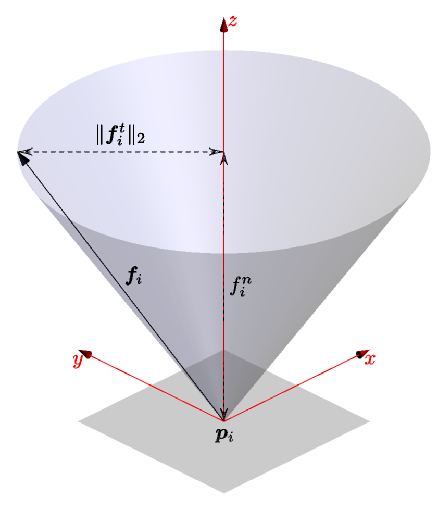
\includegraphics{friction_cone_contact.eps}}
    \caption[Friction cone and the local frame $\FRAME{i}$ of the $i$-th contact.]{
        Friction cone and the local frame $\FRAME{i}$ of the $i$-th contact.
        Square patch indicates the contact surface.
    }
    \label{fig.friction_cone_contact}
\end{figure}
%

Individual components of system~\cref{eq.complementarity_system} have the
following interpretation
\begin{description}
    \item[\cref{eq.complementarity_system.dynamics}] is the standard equation
        of dynamics of a multibody system (see \cref{app.dynamics}). The
        equation establishes relationship between motion of the joints and
        forces acting on the robot.

    \item[\cref{eq.complementarity_system.constraints}] represents constraints
        of a particular robot and setting, for example, mechanical constraints.
        These constraints are discussed later in \cref{sec.wbm_constraints}.

    \item[\cref{eq.complementarity_system.nonpenetration}] prevents
        interpenetration of the contact surface and the contacting body.

    \item[\cref{eq.complementarity_system.unilaterality}] indicates that the
        contacts are unilateral, \IE, the robot can push on the contact
        surface, but cannot pull on it.

    \item[\cref{eq.complementarity_system.complementarity}] is the
        complementarity condition, which states that a contact force cannot be
        applied at a contact surface if the contact point detaches from this
        surface.

    \item[\cref{eq.complementarity_system.frictioncone}] bounds tangential
        components of the contact force depending on the norm of its normal
        component in accordance with Coulomb's friction law.

    \item[\cref{eq.complementarity_system.frictiondirection}] indicates that
        the tangential component of the contact force is opposite to the
        sliding velocity of the contact point.
\end{description}


In order to complete the model we have to consider one more important aspect,
which manifests itself in the discrete nature of changes of the set of
contacts. These changes, or \tn{switches} of the mode of the system, indicate
that the system at hand is \tn{hybrid}. The state of such a system is often
discontinuous at the instant of a switch, and a \tn{state reinitialization
rule} must be defined \cite{Brogliato2003tranac}. In the case of the considered
system with contacts we employ an \tn{impact law} described in
\cref{app.collision} as a reinitialization rule.


%%%%%%%%%%%%%%%%%%%%%%%%%%%%%%%%%%%%%%%%%%%%%%%%%%%%%%%%%%%%%%%%%%%%%%%%%%%%%%%%
\subsection{Mechanical constraints}\label{sec.wbm_constraints}

The general inequality \cref{eq.complementarity_system.constraints} comprises
mechanical limits of the joints and motors
%
\begin{subequations}\label{eq.mechanical_constraints}
\begin{align}
    \ubar{\q}^{\prime}
    \le
    \qn
    \le
    \bar{\q}^{\prime},
    \quad
    \ubar{\dq}^{\prime}
    \le
    &
    \dqn
    \le
    \bar{\dq}^{\prime},
    \quad
    \ubar{\ddq}^{\prime}
    \le
    \ddqn
    \le
    \bar{\ddq}^{\prime}, \label{eq.joint_constraints}\\
    \ubar{\torques}
    \le
    &
    \torques
    \le
    \bar{\torques}.
\end{align}
\end{subequations}
%
In general, constraints \cref{eq.complementarity_system.constraints} are not
limited to \cref{eq.mechanical_constraints}, but such cases are not considered
in this work.


Enforcement of constraints \cref{eq.joint_constraints} is not straightforward,
when the model is used exclusively for instantaneous control. In this case, the
current state $(\q, \dq)$ is given and cannot be constrained, while the next
state is not explicitly computed. For this reason, constraints on the joint
angles and velocities are imposed through the joint accelerations. Hence,
\cref{eq.joint_constraints} boils down to \cite{Rubrecht2012auro}
%
\begin{equation}
    \ubar{\ddq}^{\prime}(\qn,\dqn)
    \le
    \ddqn
    \le
    \bar{\ddq}^{\prime}(\qn,\dqn),
\end{equation}
%
where bounds on accelerations incorporate bounds on joint angles and velocities
as well. We discuss computation of $\ubar{\ddq}^{\prime}(\qn,\dqn)$ and
$\bar{\ddq}^{\prime}(\qn,\dqn)$ in \cref{app.jointconstraints}.


%%%%%%%%%%%%%%%%%%%%%%%%%%%%%%%%%%%%%%%%%%%%%%%%%%%%%%%%%%%%%%%%%%%%%%%%%%%%%%%%
\subsection{Contact constraints and assumptions}\label{sec.contact_constraints}

One of the primary sources of nonlinearity of system
\cref{eq.complementarity_system} are the contact constraints. In order to
linearize them we make a number of approximations and assumptions. We start by
assuming that
%
\begin{description}
    \item[\ass{ass.nosliding}] There is no sliding, \IE, $\NORME{\dcontact^t_i}
        = 0$. In order to enforce this,
        constraint~\cref{eq.complementarity_system.frictiondirection}, which is
        not needed now, is replaced with
        %
        \begin{equation}\label{eq.no_tangential_acc}
            \ddcontact^t_i = \V{0}.
        \end{equation}
        %
        While being useful in manipulation~\cite{Howe1996ijrr} sliding is less
        common in locomotion~\cite{Miura2013tro}, and is usually prevented to
        simplify control.

    \item[\ass{ass.no_break_contacts}] Contacting bodies do not detach, and,
        consequently, constraint
        %
        \begin{equation}\label{eq.no_normal_acc}
            \ddcontactC^n_i = 0
        \end{equation}
        %
        must be imposed instead of nonpenetration constraint
        \cref{eq.complementarity_system.nonpenetration} and complementarity
        condition \cref{eq.complementarity_system.complementarity}. This is
        also a typical assumption. Whenever it is necessary to break one of the
        contacts, constraint \cref{eq.no_normal_acc} is replaced by a motion
        task for the contacting body.
\end{description}
%

\begin{figure}[ht]
    \begin{minipage}[t]{0.45\textwidth}
        \centering{%
        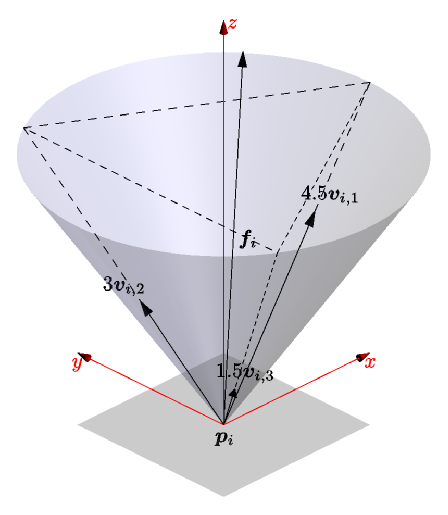
\includegraphics{friction_cone3.eps}}
        \subcaption{
            Friction cone. The force vector is represented by a weighted sum of
            vectors: $\force_i = 4.5\genvector_{i,1} + 3\genvector_{i,2} +
            1.5\genvector_{i,3}$.
        }
        \label{fig.friction_cone3}
    \end{minipage}
    \hfill
    \begin{minipage}[t]{0.45\textwidth}
        \centering{%
        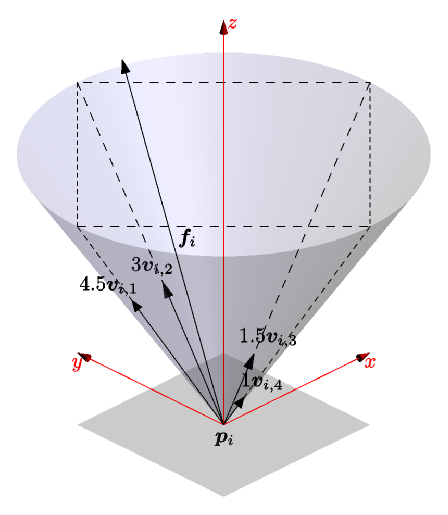
\includegraphics{friction_cone4.eps}}
        \subcaption{
            Friction cone. The force vector is represented by a weighted sum of
            vectors: $\force_i = 4.5\genvector_{i,1} + 3\genvector_{i,2} +
            1.5\genvector_{i,3} + \genvector_{i,4}$.
        }
        \label{fig.friction_cone4}
    \end{minipage}
    \caption{Linear approximation of a friction cone.}
    \label{fig.friction_cone}
\end{figure}

The next step is to linearize the quadratic
constraint~\cref{eq.complementarity_system.frictioncone}, which bounds the
$i$-th tangential contact force with respect to the normal contact force in
accordance with Coulomb's friction law. In order to linearize it, we replace
the second order cones with pyramids as shown in \cref{fig.friction_cone}. Then
for a pyramid with three faces (\cref{fig.friction_cone3}) the constraint is
expressed as
%
\begin{equation}\label{eq.friction_approx1}
    \begin{bmatrix}
        \T{(\genvector_{i,1} \CROSS \genvector_{i,2})} \\
        \T{(\genvector_{i,2} \CROSS \genvector_{i,3})} \\
        \T{(\genvector_{i,3} \CROSS \genvector_{i,1})} \\
    \end{bmatrix}
    \force_i
    \ge
    \V{0}
    ,
\end{equation}
%
where $\V{v}_{i,\{1, 2, 3\}}$ are unity vectors coinciding with the edges of
the pyramid, and cross product is used to obtain normals of the faces. Note
that \cref{eq.friction_approx1} implies unilaterality constraint
\cref{eq.complementarity_system.unilaterality} $\forceC_i^n \ge 0$, which
becomes redundant and should be removed from the system. There exist several
approaches to representation of the linearized constraints
\cite{Kuindersma2014icra}, and the one used in \cref{eq.friction_approx1} is
not optimal when it comes to solution of the system of constraints. We perform
a change of variables to express these constraints as simple bounds, which are
beneficial for solvers as indicated in \cref{sec.simple_bounds}:
%
\begin{equation}\label{eq.friction_approx2}
    \force_i
    =
    \begin{bmatrix}
        \genvector_{i,1} & \genvector_{i,2} & \genvector_{i,3}
    \end{bmatrix}
    \V{\lambda}_i
    =
    \M{V}_i
    \V{\lambda}_i,
    \quad
    \V{\lambda}_i \ge \V{0}.
\end{equation}
%


Accuracy of the linear approximation increases with the number of faces of
pyramids, which is typically chosen to be 3 or 4
(\cref{fig.friction_cone3,fig.friction_cone4} respectively). We use pyramids
with three faces, because it results in the least number of inequality
constraints.


The number of inequality constraints is further reduced by representing a foot
contact force by a single wrench $\wrench_i = (\force_i, \moment_i) =
(\M{V}_i\V{\lambda}_i, \moment_i)$ applied at $\contact_i$ instead of multiple
$3$-dimensional forces applied at several points on the foot. The force
component of the wrench is subject to Coulomb's friction constraint as above,
while the moment is constrained by
%
\begin{equation}\label{eq.moment_constraint}
    \forceC^n_i \ubar{\moment}_i \le \moment[i]_i \le  \forceC^n_i \bar{\moment}_i
    ,
    \quad
    \mbox{or}
    \quad
    \forceC^n_i \ubar{\moment}_i \le \M[][i]{R} \moment_i \le  \forceC^n_i \bar{\moment}_i
\end{equation}
%
where $\ubar{\moment}_i$ and $\bar{\moment}_i$ are constant vectors derived in
\cref{sec.rectangular_foot}, $\M[][i]{R}$ transforms the moment to the local
frame of $i$-th contact. This constraint is linear with respect to
$\V{\lambda}_i$ and $\moment_i$ and in the following is stated as
%
\begin{equation}\label{eq.moment_constraint2}
    \objA_{\moment,i}
    \begin{bmatrix}
        \V{\lambda}_i\\
        \moment_i
    \end{bmatrix}
    \ge
    \ubarV{\objb}_{\moment,i}.
\end{equation}
%


When a foot contact is represented by three or
more contact points, the orientation of the foot is fixed. In order to prevent
rotation of the foot, when the foot contact is represented by a single point
$\contact_i$, it is necessary to fix angular acceleration with the constraint
%
\begin{equation}\label{eq.no_contact_rotation}
    \dcontactW_i = \JcontactWi \ddq + \dJcontactWi \dq = \V{0}.
\end{equation}
%


%%%%%%%%%%%%%%%%%%%%%%%%%%%%%%%%%%%%%%%%%%%%%%%%%%%%%%%%%%%%%%%%%%%%%%%%%%%%%%%%
\subsection{Whole body model with linear constraints}\label{sec.linear_wbm}

Substitution of the constraints obtained in
\cref{sec.wbm_constraints,sec.contact_constraints} into the complementarity
system \cref{eq.complementarity_system} results in the whole body model with
linear constraints
%
\begin{model}{WB}{Whole Body}
\begin{subequations}\label{eq.linearized_system}
\begin{empheq}[left=\empheqlbrace]{align}
    & \M{H} \ddq + \V{h} = \Itorques\torques + m\T{\Jcom} \V{g} + \sum_{i=1}^M \T{\M{J}_i} \wrench_i
        ,
        \\
    &
        \begin{bmatrix}
            \ddcontact_i \\
            \dcontactW_i
        \end{bmatrix}
        =
        \begin{bmatrix}
            \Jcontacti \\
            \JcontactWi
        \end{bmatrix}
        \ddq
        +
        \begin{bmatrix}
            \dJcontacti \dq \\
            \dJcontactWi \dq
        \end{bmatrix}
        =
        \M{J}_i
        \ddq
        +
        \dotM{J}_i
        \dq
        =
        \V{0}
        ,
        \label{eq.linearized_system.fixedcontact}
        \\
    & \ubar{\torques}  \le  \torques  \le  \bar{\torques}
        ,
        \label{eq.linearized_system.ctrtorques}
        \\
    & \ubar{\ddq}^{\prime}  \le  \ddqn  \le  \bar{\ddq}^{\prime}
        ,
        \label{eq.linearized_system.ctrq}
        \\
    &
        \objA_{\moment,i}
        \begin{bmatrix}
            \V{\lambda}_i\\
            \moment_i
        \end{bmatrix}
        \ge
        \ubarV{\objb}_{\moment,i}
        \label{eq.linearized_system.moments}
        ,
        \\
    &
        \V{\lambda}_i \ge \V{0}
        ,
        \label{eq.linearized_system.friction}
\end{empheq}
\end{subequations}
\end{model}
%
where $\wrench_i = (\force_i, \moment_i) = (\M{V}_i\V{\lambda}_i, \moment_i)$,
$\M{J}_i$ is the contact point Jacobian including both translational and
rotational parts. Dependence of $\M{H}$, $\V{h}$, $\ubar{\ddq}^{\prime}$,
$\bar{\ddq}^{\prime}$, and Jacobians on $\q$ and $\dq$ is omitted for brevity.
Equation \cref{eq.linearized_system.fixedcontact} incorporates constraints
\cref{eq.no_tangential_acc}, \cref{eq.no_normal_acc}, and
\cref{eq.no_contact_rotation}.



%%%%%%%%%%%%%%%%%%%%%%%%%%%%%%%%%%%%%%%%%%%%%%%%%%%%%%%%%%%%%%%%%%%%%%%%%%%%%%%%
\subsection{Controlling the robot}\label{sec.wbm_control}

The primary interest of our modeling effort is to allow control of a humanoid
robot using its model. It turns out, that we have already introduced elements
of control in \nameref{model.WB} model by adding constraint
%
\begin{equation}\label{eq.fixed_position}
    \ddcontact_i = \Jcontacti \ddq + \dJcontacti \dq = \V{0}
\end{equation}
%
in order to support \cref{ass.nosliding,ass.no_break_contacts}. This constraint
is clearly not physical, but rather dictated by our control goals. It falls
within the framework of \tn{operational space control} \cite{Khatib1987jra} or
more general \tn{task function control approach}
\cite[Chapter~3]{Samson1991robot}, both of which focus on control of the
end-effectors of the robot rather than its joints. Hence, we call
\cref{eq.fixed_position} a \tn{task}, whose purpose is to maintain constant
position of the end-effector corresponding to the contact point. In a similar
way we define tasks for other parts of the robot's body
%
\begin{equation}
    \M{J}_{\!\MT{ee}}\ddq + \dotM{J}_{\!\MT{ee}} \dq = \ddotV{y}^{\DES}_{\!\MT{ee}},
\end{equation}
%
where $\M{J}_{\!\MT{ee}}$ and $\ddotV{y}^{\DES}_{\!\MT{ee}}$ are the Jacobian
and the desired acceleration of a certain end-effector.
$\ddotV{y}^{\DES}_{\!\MT{ee}}$ can be obtained with a simple
\acs{PD}-controller such as
%
\begin{equation}
    \ddotV{y}^{\DES}_{\!\MT{ee}}
    =
    \K_{p,\MT{ee}} (\V{y}^{\DES}_{\!\MT{ee}} - \V{y}_{\!\MT{ee}})
    -
    \K_{d,\MT{ee}} \dotV{y}_{\!\MT{ee}},
\end{equation}
%
which drives the end-effector to the desired position
$\V{y}^{\DES}_{\!\MT{ee}}$ given current position $\V{y}$ and velocity
$\dotV{y}$, and positive scalar gains $\K_{p,\MT{ee}}$, $\K_{d,\MT{ee}}$.
Examples of various end-effector tasks for humanoid robots can be found in
\cite[Chapter~4]{Kanoun2009thesis}.


Tasks, however, are not limited to control of the end-effectors. For example,
the joint-level task
%
\begin{equation}
    \ddqn = \K_{p,\qn} (\qn[\DES] - \qn) - \K_{d,\qn} \dqn
\end{equation}
%
employs a \acs{PD}-controller to maintain the desired joint configuration
$\qn[\DES]$. Furthermore, tasks can also be posed as inequalities
\cite[Chapter~3]{Kanoun2009thesis}
%
\begin{equation}
    \ubar{\ddotV{y}}_{\!\MT{ee}}
    \le
    \M{J}_{\!\MT{ee}}\ddq + \dotM{J}_{\!\MT{ee}} \dq
    \le
    \bar{\ddotV{y}}_{\!\MT{ee}}.
\end{equation}
%
Thus, we conclude that the difference between tasks and constraints in the
model is only a matter of interpretation: as we are going to see in
\cref{ch.optimization}, the only important thing for numerical computations is
prioritization of the constraints or tasks with respect to each other. Hence,
in the following we use terms ``task'' and ``constraint'' interchangeably.


All whole body motion controllers employed in this work include tasks for
control of motion of the \ac{CoM} and orientation of the body, which are
related to linear and angular momenta respectively. Both are important for
balance preservation: in order to stop the robot it is necessary to nullify its
momenta. Furthermore, control over vertical motion of the \ac{CoM} helps to
prevent falls, which cannot be prevented by the constraints in
\nameref{model.WB} model. The desired values for momenta are obtained by
anticipating the motion of the robot with approximate linear models described
later in this chapter.


While controlling the robot using the task function approach, we may encounter
several types of problems. The first problem arises when imposed tasks do not
require all degrees of freedom of the system. This implies that the robot is
\tn{redundant} with respect to the tasks and there is an infinite number of
control inputs that achieve our goals \cite[Chapter~4]{Samson1991robot}. We can
easily alleviate this issue by adding tasks, which, however, increase the
chance of triggering the second problem: a \tn{conflict} of the tasks with each
other and the physical constraints. Both redundancy and conflicts are important
subjects of this thesis and are discussed in \cref{ch.optimization}. Another
important question is dealing with online addition, removal, or transformation
of the tasks, which is not considered here \cite{Lee2012tro}.



%%%%%%%%%%%%%%%%%%%%%%%%%%%%%%%%%%%%%%%%%%%%%%%%%%%%%%%%%%%%%%%%%%%%%%%%%%%%%%%%
%%%%%%%%%%%%%%%%%%%%%%%%%%%%%%%%%%%%%%%%%%%%%%%%%%%%%%%%%%%%%%%%%%%%%%%%%%%%%%%%
%%%%%%%%%%%%%%%%%%%%%%%%%%%%%%%%%%%%%%%%%%%%%%%%%%%%%%%%%%%%%%%%%%%%%%%%%%%%%%%%
\section{Nonlinear approximate models}\label{sec.nonlinear_approx_models}

The whole body (\nameref{model.WB}) model reviewed in
\cref{sec.whole_body_model} allows for the control of the robot, but it varies
nonlinearly with the state of the system and is rather complicated. We have
already indicated in \cref{sec.balance_general}, that such complexity is not
always needed when online motion anticipation is performed. In this case it is
common to employ approximate models, which are derived from the complete model
under certain assumptions. In the present section we consider two approximate
nonlinear models, which we do not employ \tn{per se}, but use them later in
\cref{sec.linear_approx_models} for the construction of linear models.


%%%%%%%%%%%%%%%%%%%%%%%%%%%%%%%%%%%%%%%%%%%%%%%%%%%%%%%%%%%%%%%%%%%%%%%%%%%%%%%%
\subsection{Nonlinear momenta-based model}\label{sec.momenta_based_nonlinear}

First, let us consider the friction constraints
\cref{eq.linearized_system.moments}, \cref{eq.linearized_system.friction} in
\nameref{model.WB} model. It is interesting to observe that they primarily
limit the aggregate motion of the robot, \IE, the rate of its spatial momentum.
That is, as long as the rate of momentum complies with these constraints, the
joint motion can be arbitrary, provided that the motors can produce sufficient
torques and joint limits are satisfied. We demonstrate this by rewriting the
equation of dynamics using derivations from \cref{app.dynamics} as
%
\begin{equation}
    \underbrace{
        \begin{bmatrix}
            \M{H}_1\\
            \M{H}_2\\
            \M{H}_3\\
        \end{bmatrix}
    }_{\M{H}}
    \underbrace{
        \begin{bmatrix}
            \ddqn\\
            \ddotV{r}\\
            \ddotV{\EULER}
        \end{bmatrix}
    }_{\ddq}
    +
    \underbrace{
        \begin{bmatrix}
            \V{h}_1\\
            \V{h}_2\\
            \V{h}_3
        \end{bmatrix}
    }_{\V{h}}
    =
    \begin{bmatrix}
        \torques\\
        \V{0}\\
        \V{0}
    \end{bmatrix}
    +
    m
    \underbrace{
        \begin{bmatrix}
            \T{\Jcom[,1]}\\
            \T{\Jcom[,2]}\\
            \T{\Jcom[,3]}
        \end{bmatrix}
    }_{\T{\Jcom}}
    \V{g}
    +
    \sum_{i=1}^M
    \underbrace{
        \begin{bmatrix}
            \T{\M{J}_{i,1}}\\
            \T{\M{J}_{i,2}}\\
            \T{\M{J}_{i,3}}
        \end{bmatrix}
    }_{\T{{\M{J}}_i}}
    \wrench_i,
\end{equation}
%
and use the first line of this equation to eliminate $\torques$ from
\nameref{model.WB} model to obtain
%
\begin{subequations}\label{eq.eliminated_torques}
\begin{empheq}[left=\empheqlbrace]{align}
    &   \begin{bmatrix}
            \M{I}   &   \M{0} \\
            \M{0}   &   \T{\Teuler}\\
        \end{bmatrix}
        \begin{bmatrix}
            \dotV[r]{\LM} \\
            \dotV[r]{\AM}\\
        \end{bmatrix}
        =
        \begin{bmatrix}
            \M{H}_2\\
            \M{H}_3\\
        \end{bmatrix}
        \ddq
        +
        \begin{bmatrix}
            \V{h}_2\\
            \V{h}_3
        \end{bmatrix}
        =
        m
        \begin{bmatrix}
            \T{\Jcom[,2]}\\
            \T{\Jcom[,3]}
        \end{bmatrix}
        \V{g}
        +
        \sum_{i=1}^M
            \begin{bmatrix}
                \T{\M{J}_{i,2}}\\
                \T{\M{J}_{i,3}}
            \end{bmatrix}
        \begin{bmatrix}
            \force_i\\
            \moment_i
        \end{bmatrix},
        ,
        \\
    &   \begin{bmatrix}
            \ddcontact_i \\
            \dcontactW_i
        \end{bmatrix}
        =
        \M{J}_i
        \ddq
        +
        \dotM{J}_i
        \dq
        =
        \V{0}
        ,
        \label{eq.eliminated_torques.fixedcontact}
        \\
    &
        \force_i
        =
        \M{V}_i
        \V{\lambda}_i
        ,
        \\
    &   \ubar{\torques}
        \le
        \M{H}_1 \ddq  +  \V{h}_1  -  m \T{\Jcom[,1]} \V{g}  -  \sum_{i=1}^M \T{\M{J}_{i,1}}
        \begin{bmatrix}
            \force_i\\
            \moment_i
        \end{bmatrix}
        \le
        \bar{\torques}
        ,
        \label{eq.eliminated_torques.ctrtorques}
        \\
    & \ubar{\ddq}^{\prime}  \le  \ddqn  \le  \bar{\ddq}^{\prime}
        ,
        \label{eq.eliminated_torques.ctrq}
        \\
    &
        \objA_{\moment,i}
        \begin{bmatrix}
            \V{\lambda}_i\\
            \moment_i
        \end{bmatrix}
        \ge
        \ubarV{\objb}_{\moment,i}
        ,
        \\
    & \V{\lambda}_i \ge \V{0},
        \label{eq.eliminated_torques.friction}
\end{empheq}
\end{subequations}
%
where $\dotV[r]{\LM}$ and $\dotV[r]{\AM}$ are rates of linear and angular
momenta respectively, and $\Teuler$ transforms derivatives of the Euler angles
to angular velocities (see \cref{sec.jacobians}). Assuming that
%
\begin{description}
    \item[\ass{ass.nojointctr}] constraints of the joints and motors
        \cref{eq.eliminated_torques.ctrtorques},
        \cref{eq.eliminated_torques.ctrq}, and contact preservation task
        \cref{eq.eliminated_torques.fixedcontact} are always satisfied,
\end{description}
%
we neglect the structure of the robot and focus on its momenta and contact
forces. Both the contact forces and momenta are crucial for ensuring balance in
motion anticipation: control over the former allows to avoid tipping and
slipping, over the latter -- to stop motion of the robot as indicated in
\cref{sec.wbm_control}. Under \cref{ass.nojointctr} the model boils down to
constrained Newton-Euler equations for a rigid body (see also
\cref{app.dynamics})
%
\begin{model}{NMB}{Nonlinear Momenta-Based}
\begin{subequations}\label{eq.simplified_system}
\begin{empheq}[left=\empheqlbrace]{align}
    &   \begin{bmatrix}
            \dotV[r]{\LM} \\
            \dotV[r]{\AM}\\
        \end{bmatrix}
        =
        m
        \begin{bmatrix}
            \M{I} \\
            \CROSS[(\V{c} - \V{r})]
        \end{bmatrix}
        \V{g}
        +
        \sum_{i=1}^M
            \begin{bmatrix}
                \M{I}                     & \M{0}\\
                \CROSS[(\contact_i - \V{r})]   & \M{I}
            \end{bmatrix}
            \begin{bmatrix}
                \force_i\\
                \moment_i
            \end{bmatrix},
        \label{eq.simplified_system.dynamics}\\
    & \force_i = \M{V}_i \V{\lambda}_i,
      \\
    &
        \objA_{\moment,i}
        \begin{bmatrix}
            \V{\lambda}_i\\
            \moment_i
        \end{bmatrix}
        \ge
        \ubarV{\objb}_{\moment,i}
        ,
        \\
    & \V{\lambda}_i \ge \V{0},
        \label{eq.simplified_system.friction}\\
    & \mbox{proxy constraints}.
        \label{eq.simplified_system.fixedcontact}
\end{empheq}
\end{subequations}
\end{model}
%
Here, the term \tn{proxy constraints} is used as in
\cite[Chapter~3]{Zaytsev2015thesis} and denotes constraints, which allow to
take into account \cref{eq.eliminated_torques.ctrtorques},
\cref{eq.eliminated_torques.ctrq}, and
\cref{eq.eliminated_torques.fixedcontact} indirectly through the variables
still present in \nameref{model.NMB} model. For example, one may choose to
reflect kinematic limits of the robot by constraining distance between \ac{CoM}
$\V{c}$ and contact points $\contact_i$. Proxy constraints are typically rough
approximations, but are often necessary to support \cref{ass.nojointctr}.


Equation \cref{eq.simplified_system.dynamics} has several properties, which
are important to mention:
%
\begin{itemize}
    \item It is more convenient to work with Newton-Euler equation when the
        base position coincides with the \ac{CoM} $\V{c} = \V{r}$ resulting in
        %
        \begin{equation}
            \begin{bmatrix}
                \dotV[c]{\LM} \\
                \dotV[c]{\AM}\\
            \end{bmatrix}
            =
            \begin{bmatrix}
                m\V{g}\\
                \V{0}
            \end{bmatrix}
            +
            \sum_{i=1}^M
                \begin{bmatrix}
                    \M{I}                     & \M{0}\\
                    \CROSS[(\contact_i - \V{c})]   & \M{I}
                \end{bmatrix}
                \begin{bmatrix}
                    \force_i\\
                    \moment_i
                \end{bmatrix}.
        \end{equation}
        %

    \item Another important property of \cref{eq.simplified_system.dynamics} is
        nonholonomy of its lower part corresponding to the rate of angular
        momentum \cite{Wieber2006fastmotions}. This means that
        \cref{eq.simplified_system.dynamics} constrains rotational motion of
        the system, but not its orientation. The best known illustration of
        this fact is a falling cat (see \cref{fig.falling_cat}), which changes
        its orientation in mid-air without using any contacts with the
        environment to finally land on its paws. Since there is no clear
        connection between orientation of the robot and its angular momentum,
        it is also unclear what are the desired values for angular momentum. It
        is presumed that the angular momentum should be kept small, but not
        equal to zero \cite{Wieber2006fastmotions}. In the present work, we
        constrain the angular momentum by including it in a capturability
        constraint (see \cref{sec.momenta_model_capturability}). Though not
        necessary in our simulations, it is also reasonable to bound it.
        %
        \begin{figure}[ht]
            \centering{%
            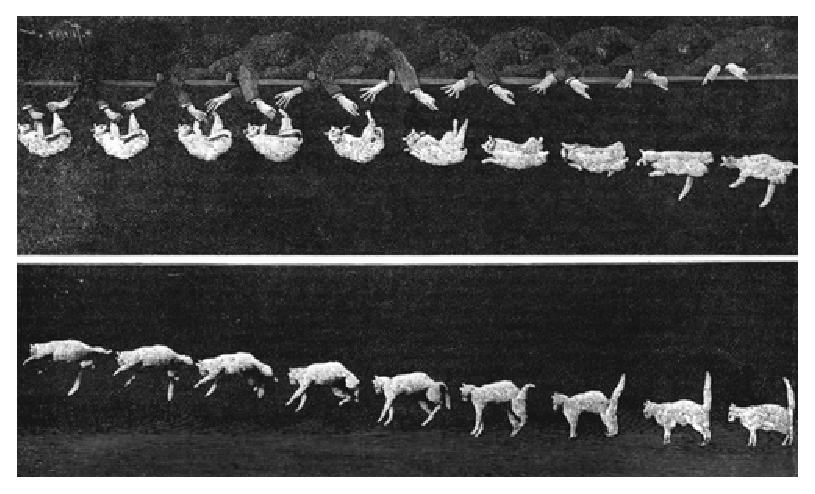
\includegraphics{Falling_cat_1894.eps}}
            \caption[Cat is changing its orientation during a fall to land on its paws.]{
                Cat changes its orientation while falling even though its
                angular momentum is initially zero and conserved during a fall.
                Snapshots of a short film recorded by \'Etienne-Jules Marey in
                1894 \cite{FallingCat}.
            }
            \label{fig.falling_cat}
        \end{figure}
\end{itemize}
%


%%%%%%%%%%%%%%%%%%%%%%%%%%%%%%%%%%%%%%%%%%%%%%%%%%%%%%%%%%%%%%%%%%%%%%%%%%%%%%%%
\subsection{Nonlinear point-mass model}\label{sec.point_mass_nonlinear}

In order to construct this model we introduce additional assumptions. Also, we
facilitate derivations by manipulating the position and orientation of the
global frame. In practice, however, it may be more convenient to utilize models
in convenient working frames and transform data to the global frame when
necessary. In many cases it is beneficial to choose the orientation of the
global (working) frame so that
%
\begin{description}
    \item[\ass{ass.gravity_z_aligned}] its $z$ axis is parallel to the gravity
        vector $\V{g}$, \IE, $\V{g}^{xy} = \V{0}$.
\end{description}
%
Also, we simplify derivations by taking the orientation of $\FRAME{c}$ to be
the same as the orientation of the global (working) frame, \IE, $\V{\LM} =
\V[c]{\LM}$ and $\dotV{\LM} = \dotV[c]{\LM}$.


The characteristic feature of the point-mass model is the absence of angular
momentum $\V[c]{\AM} = \V{0}$, since all the mass of the robot is concentrated
in a point. Note that in spite of the popularity of such point-mass
approximations, it is not strictly necessary to neglect angular momentum to
construct a linear model.

We start with \nameref{model.NMB} model, but this time we express it with
respect to the global (working) frame
%
\begin{subequations}\label{eq.simplified_system1}
\begin{empheq}[left=\empheqlbrace]{align}
    &
        \begin{bmatrix}
            \dotV{\LM} \\
            \dotV{\AM}
        \end{bmatrix}
        =
        \begin{bmatrix}
            \dotV[c]{\LM} \\
            \dotV[c]{\AM} + \V{c} \CROSS \dotV[c]{\LM}\\
        \end{bmatrix}
        =
        \begin{bmatrix}
            m \ddotV{c} \\
            \dotV[c]{\AM} + m \V{c} \CROSS \ddotV{c}\\
        \end{bmatrix}
        =
        \begin{bmatrix}
            m\V{g}\\
            m \V{c} \CROSS \V{g}
        \end{bmatrix}
        +
        \sum_{i=1}^M
            \begin{bmatrix}
                \M{I}             & \M{0}\\
                \CROSS[\contact_i]  & \M{I}
            \end{bmatrix}
            \begin{bmatrix}
                \force_i\\
                \moment_i
            \end{bmatrix}
        ,
        \label{eq.simplified_system1.dynamics}\\
    & \force_i = \M{V}_i \V{\lambda}_i,
        \\
    &
        \objA_{\moment,i}
        \begin{bmatrix}
            \V{\lambda}_i\\
            \moment_i
        \end{bmatrix}
        \ge
        \ubarV{\objb}_{\moment,i}
        ,
        \label{eq.simplified_system1.moments}
        \\
    & \V{\lambda}_i \ge \V{0},
        \label{eq.simplified_system1.friction}
        \\
    & \mbox{proxy constraints}.
        \label{eq.simplified_system1.fixedcontact}
\end{empheq}
\end{subequations}
%
Then we assume that
%
\begin{description}
    \item[\ass{ass.coplanar_contacts}] the support (ground) surface is flat, is
        spanned by $x$ and $y$ axes of the global (working) frame, and intersects $z$
        axis at $\contactC^z$,
\end{description}
%
and divide the set of all contacts into two groups:
%
\begin{enumerate}
    \item one contains all $\{1, ..., M_s\}$ support contacts, such that
        $\contactC^z_i = \contactC^z$;

    \item another contains all remaining contacts.
\end{enumerate}
%
For simplicity, all forces corresponding to the contacts of the second group
are reduced to a single wrench $(\forceext, \momentext)$ acting on the
\ac{CoM}. This wrench is used, for example, to model interaction with a
human-collaborator \cite{Agravante2016icra}, but usually it is taken to be zero.
Once this is done, the equation for the rates of momenta is transformed to
%
\begin{subequations}
    \begin{empheq}[left=\empheqlbrace]{align}
        &
        m
        \ddotV{c}
        -
        m
        \V{g}
        -
        \forceext
        =
        \sum_{i = 1}^{M_s}
        \force_i
        =
        \force_s
        \\
        &
        \dotV[c]{\AM}
        +
        \V{c}
        \CROSS
        \force_s
        -
        \momentext
        =
        \sum_{i=1}^{M_s}
        \left(
            \contact_i
            \CROSS
            \force_i
            +
            \moment_i
        \right),
    \end{empheq}
\end{subequations}
%
where $\force_s$ is the total support surface reaction force. Each contact
position can be represented by a sum of two vectors $\contact_i =
(\contact_i^{xy}, 0) + (\V{0}, \contactC^z)$, hence
%
\begin{equation}\label{eq.contact_height}
    \sum_{i=1}^{M_s}
        \contact_i
        \CROSS
        \force_i
    =
    \begin{bmatrix}
        \V{0}\\
        \contactC^z
    \end{bmatrix}
    \CROSS
    \underbrace{
    \left(
    \sum_{i=1}^{M_s}
        \force_i
    \right)}_{\force_s}
    +
    \sum_{i=1}^{M_s}
        \begin{bmatrix}
            \contact_i^{xy}\\
            0
        \end{bmatrix}
        \CROSS
        \force_i\\
\end{equation}
%

Substitution of \cref{eq.contact_height} into the equation for the rate of
angular momentum yields
%
\begin{equation}
    \dotV[c]{\AM}
    +
    \begin{bmatrix}
        0      &   \contactC^z - c^z  &   c^y\\
        c^z - \contactC^z   &   0      &   -c^x\\
        -c^y   &   c^x    &   0 \\
    \end{bmatrix}
    \force_s
    -
    \momentext
    =
    \sum_{i=1}^{M_s}
    \left(
        \begin{bmatrix}
            0               &   0               &   \contactC_i^y\\
            0               &   0               &   -\contactC_i^x\\
            -\contactC_i^y  &   \contactC_i^x   &   0 \\
        \end{bmatrix}
        \force_i
        +
        \moment_i
    \right).
\end{equation}
%
We avoid nonlinearity of this equation by assuming that
%
\begin{description}
    \item[\ass{ass.arbitrary_z_moment}] moments about the $z$ axis
        $\momentC_i^z$ can be arbitrary and the $z$ component of constraint
        \cref{eq.simplified_system1.moments} can be omitted.
\end{description}
%
Then $\dotC[c]{\AM}^z$ can be always set to any desired value, for example
zero, and the respective equation can be neglected. Provided that
%
\begin{description}
    \item[\ass{ass.nonzero_z_force}] $\forceC_s^z \ne 0$, which implies $m
        \ddotC{c}^z \ne m \C{g}^z + \forceextC^z$, \IE, the robot interacts
        with the support surface,
\end{description}
%
we divide the remaining equations for the rates of angular momentum by the
total vertical force $\forceC_s^z$
%
\begin{equation}
    \setlength{\arraycolsep}{2pt}
    \frac{
        1
    }
    {
        \forceC_s^z
    }
    \left(
        \dotC[c]{\AM}^{xy} \\
        +
        \begin{bmatrix}
            0      &   \contactC^z -c^z   &   c^y\\
            c^z - \contactC^z   &   0      &   -c^x\\
        \end{bmatrix}
        \force_s
        -
        \momentext^{xy}
    \right)
    =
    \frac{
        1
    }
    {
        \forceC_s^z
    }
        \sum_{i=1}^{M_s}
        \left(
            \forceC_i^z
            \begin{bmatrix}
                \contactC_i^y  \\
                -\contactC_i^x \\
            \end{bmatrix}
            +
            \moment_i^{xy} \\
        \right)
    =
    \frac{
        \moment_{s}^{xy} \\
    }
    {
        \forceC_s^z
    }
\end{equation}
%
where $\moment_{s}^{xy}$ is the total moment created by the surface contacts.
Then the rightmost expression is equal to $(\copC^y, -\copC^x)$ as shown in
\cref{sec.rectangular_foot}, and $(\copC^x, \copC^y)$ is the position of the
\ac{CoP} of all support contacts. In this context the \ac{CoP} is also known as
\ac{ZMP}, since the moments about the $x$ and $y$ axes are zero in this point
\cite{Vukobratovic2004ijhr}. The \ac{CoP} must stay within the \tn{support
area} -- the convex hull of all support contacts illustrated in
\cref{fig.support_area}: $\cop \in \SET{S}(\contact_1^{xy}, ...
,\contact_{M_s}^{xy})$. This constraint on the position of the \ac{CoP} is
equivalent to the remaining constraints on $x$ and $y$ components of contact
moments in \cref{eq.simplified_system1.moments} as follows from
\cref{sec.rectangular_foot,sec.surface_contacts}.


\begin{figure}[ht]
    \centering{%
    \includegraphics{support_area.eps}}
    \caption[Support area of two rectangular feet.]{
        Grey area represents support area $\SET{S}(\contact_1^{xy},
        \contact_2^{xy})$ of two rectangular foot contacts.
    }
    \label{fig.support_area}
\end{figure}


Now we drop individual support contact forces and moments $(\force_i,
\moment_i)$ with $i \in \{1, ..., M_s\}$ to obtain
%
\begin{subequations}\label{eq.no_ground_contact_forces}
    \begin{empheq}[left=\empheqlbrace]{align}
        &
            \force_s
            =
            m
            (\ddotV{c} - \V{g})
            -
            \forceext
            =
            \sum_{i = 1}^{M_s}
                \M{V}_i \V{\lambda}_i
            ,
            \\
        &
            \frac{1}{\forceC_s^z}
            \left(
                \dotV[c]{\AM}^{xy}
                -
                \momentext^{xy}
                -
                (
                    c^z
                    -
                    \contactC^z
                )
                \begin{bmatrix}
                    \forceC_s^y \\
                    -\forceC_s^x\\
                \end{bmatrix}
            \right)
            +
            \begin{bmatrix}
                c^y\\
                -c^x\\
            \end{bmatrix}
            =
            \begin{bmatrix}
                \copC^y\\
                -\copC^x
            \end{bmatrix},
            \\[2mm]
        &
            \cop \in \SET{S}(\contact_1^{xy}, ... ,\contact_{M_s}^{xy})
            ,
            \\
        & \V{\lambda}_i \ge \V{0},
            \\
        & \forceC_s^z \ne 0,
            \label{eq.no_ground_contact_forces.nonzero_z_force}
            \\
        & \mbox{proxy constraints}.
    \end{empheq}
\end{subequations}
%
The system is further simplified if
%
\begin{description}
    \item[\ass{ass.point_mass}] The rate of angular momentum is always zero
        $\V[c]{\AM}^{xy} = \V{0}$, which implies that the system models a
        point-mass. This is an ubiquitous assumption in the literature, even
        though it is not required to construct a linear model
        \cite{Wieber2015handbook}.

    \item[\ass{ass.same_friction}] The friction coefficients are the same for
        all contacts, so that $\M{V}_i = \M{V}$ and
        %
        $
            \force_s = \V{V} \sum_{i = 1}^{M_s} \V{\lambda}_i
            \quad
            \mbox{or}
            \quad
            \force_s = \M{V} \V{\lambda}
        $
        %
        with $\V{\lambda} \ge \V{0}$, which makes variables $\V{\lambda}_i$
        unnecessary.
\end{description}
%
\cref{ass.same_friction} implies that the total surface contact force is
constrained to the same friction cone as individual surface contact forces.


Thus, the system takes the following form
%
\begin{model}{NPM}{Nonlinear Point-Mass}
\begin{subequations}\label{eq.nonlinear_point_mass}
    \begin{empheq}[left=\empheqlbrace]{align}
        &
            \cop
            =
            \V{c}^{xy}
            -
            \zeta
            \force_s^{xy} / m
            +
            \frac{1}{\forceC_s^z}
            \begin{bmatrix}
                - \momentextC^y \\
                \momentextC^x \\
            \end{bmatrix}
            ,
            \\
        &
            \zeta
            =
            \frac{m (c^z - \contactC^z)}{\forceC_s^z}
            ,
            \\[2mm]
        &
            \cop \in \SET{S}(\contact_1^{xy}, ... ,\contact_{M_s}^{xy})
            ,
            \label{eq.nonlinear_point_mass.cop_ctr}
            \\
        & \forceC_s^z \ne 0,
            \label{eq.nonlinear_point_mass.nonzero_z_force}
            \\
        &
            \force_s
            =
            m
            (\ddotV{c} - \V{g})
            -
            \forceext
            =
            \M{V} \V{\lambda}
            ,
            \quad
            \V{\lambda} \ge \V{0}
            ,
            \label{eq.nonlinear_point_mass.friction}
            \\
        & \mbox{proxy constraints}
            ,
            \label{eq.nonlinear_point_mass.proxy}
    \end{empheq}
\end{subequations}
\end{model}
%
where the first equation is nonlinear with respect to motion of the \ac{CoM}
and external force $\forceext$, and constraint
\cref{eq.nonlinear_point_mass.cop_ctr} is nonlinear with respect to positions
and orientations of the contacts as explained in \cref{sec.surface_contacts}.



%%%%%%%%%%%%%%%%%%%%%%%%%%%%%%%%%%%%%%%%%%%%%%%%%%%%%%%%%%%%%%%%%%%%%%%%%%%%%%%%
%%%%%%%%%%%%%%%%%%%%%%%%%%%%%%%%%%%%%%%%%%%%%%%%%%%%%%%%%%%%%%%%%%%%%%%%%%%%%%%%
%%%%%%%%%%%%%%%%%%%%%%%%%%%%%%%%%%%%%%%%%%%%%%%%%%%%%%%%%%%%%%%%%%%%%%%%%%%%%%%%
\section{Linear approximate models}\label{sec.linear_approx_models}

In the present work we employ two types of approximate models: the first one
(\cref{sec.model_momenta}) is tailored for 3-dimensional multi-contact
settings, the second (\cref{sec.point_mass_planar,sec.point_mass_nonplanar}) --
for walking. All of these models are based on the models described in
\cref{sec.nonlinear_approx_models} and are linear. Though nonlinear models find
more and more applications in practice, they are generally more demanding for
computational resources \cite{Koenemann2015iros}.



%%%%%%%%%%%%%%%%%%%%%%%%%%%%%%%%%%%%%%%%%%%%%%%%%%%%%%%%%%%%%%%%%%%%%%%%%%%%%%%%
\subsection{Momenta-based model with noncoplanar contacts}\label{sec.model_momenta}

The linear model for preview of linear and angular momenta derived in this
section was originally proposed in \cite{Nagasaka2012} in Japanese and later
restated with some minor extensions in \cite{Audren2014iros,
Sherikov2015humanoids} in English.


The component-wise equation of rate of angular momentum in \nameref{model.NMB}
model has the following form
%
\begin{equation}\label{eq.component_wise_momenta}
    \begin{bmatrix}
        \dotC[c]{\AM}^x\\
        \dotC[c]{\AM}^y\\
        \dotC[c]{\AM}^z
    \end{bmatrix}
    =
    \sum_{i=1}^M
    \left(
        \begin{bmatrix}
            0                   & - (\contactC_i^z - {c}^z)   & \contactC_i^y - {c}^y \\
            \contactC_i^z - {c}^z     & 0                     & - (\contactC_i^x - {c}^x)\\
            - (\contactC_i^y - {c}^y) & \contactC_i^x - {c}^x       & 0
        \end{bmatrix}
        \begin{bmatrix}
            \forceC_i^x\\
            \forceC_i^y\\
            \forceC_i^z
        \end{bmatrix}
        +
        \begin{bmatrix}
            \momentC_i^x\\
            \momentC_i^y\\
            \momentC_i^z
        \end{bmatrix}
    \right).
\end{equation}
%
In order to avoid nonlinearity in this equation we assume that
%
\begin{description}
    \item[\ass{ass.fixed_points}] Contact points $\contact_i$ are given constants.

    \item[\ass{ass.fixed_z_coordinate}] $\C{c}^z$ is a given constant, which
        implies that the \ac{CoM} acceleration along the $z$ axis is zero and
        %
        \begin{equation}
            \dotC{\LM}^z
            =
            m
            \ddot{c}^z
            =
            m
            g^z
            +
            \sum_{i=1}^M
                \forceC_i^z
            =
            0.
        \end{equation}
        %

    \item[\ass{ass.arbitrary_z_momentum}] Rate of angular momentum about the
        $z$ axis is arbitrary. In other words, the computed rotational motion
        about the $z$ axis is always feasible. Validity of this assumption is
        not completely clear, but no problems in simulations were reported so
        far. This assumption is opposite to \cref{ass.arbitrary_z_moment},
        which allows for arbitrary contact moments about the $z$ axis in the
        point-mass (\nameref{model.NPM}) model.
\end{description}
%


Since the vertical motion of the \ac{CoM} is prohibited by
\cref{ass.fixed_z_coordinate} and $\dotC[c]{\AM}^z$ is neglected due to
\cref{ass.arbitrary_z_momentum}, we focus on the linear and angular momenta
about the $x$ and $y$ axes:
%
\begin{align}\label{eq.dynamics_momenta_model}
    \dotV{\LM}^{xy}
    &
    =
    m
    \ddotV{c}^{xy}
    =
    \underbrace{
        m
        \V{g}^{xy}
    }_{\tildeV{b}}
    +
    \sum_{i=1}^M
        \force_i^{xy}
    \\
    \dotV[c]{\AM}^{xy}
    &
    =
    \sum_{i=1}^M
    \Bigg(
        \underbrace{
            \begin{bmatrix}
                0                   & - (\contactC_i^z - {c}^z)   & \contactC_i^y\\
                \contactC_i^z - {c}^z     & 0                     & - \contactC_i^x\\
            \end{bmatrix}
        }_{\tildeM{B}_{i}}
        \force_i
        +
        \Ixy
        \moment_i
    \Bigg)
    +
    \underbrace{
        \begin{bmatrix}
            0     &     g^z \\
            - g^z &     0
        \end{bmatrix}
    }_{\tildeM{A}}
    \underbrace{
        (
            m \V{c}^{xy}
        )
    }_{\hatV{\LM}^{xy}}
\end{align}
%
Then we construct a linear continuous-time model with $M$ control inputs
$\wrench_i = (\force_i, \moment_i)$ and state vector $\V{x} = (m \V{c}^{xy},
\V{\LM}^{xy}, \V[c]{\AM}^{xy}) = (\hatV{\LM}^{xy}, \V{\LM}^{xy},
\V[c]{\AM}^{xy})$:
%
\begin{model}{CMB}{Continuous Momenta-Based}
\begin{subequations}\label{eq.continuous_momenta_model}
\begin{empheq}[left=\empheqlbrace]{align}
    &
        \underbrace{
            \begin{bmatrix}
                \V{\LM}^{xy}\\
                \dotV{\LM}^{xy}\\
                \dotV[c]{\AM}^{xy}
            \end{bmatrix}
        }_{\dotV{x}}
        =
        \underbrace{
            \begin{bmatrix}
                \V{0}         & \V{I}   & \V{0}\\
                \V{0}         & \V{0}   & \V{0}\\
                \tildeM{A}  & \V{0}   & \V{0}
            \end{bmatrix}
        }_{\M{A}}
        \underbrace{
            \begin{bmatrix}
                \hatV{\LM}^{xy}\\
                \V{\LM}^{xy}\\
                \V[c]{\AM}^{xy}
            \end{bmatrix}
        }_{\V{x}}
        +
        \sum_{i=1}^M
        \underbrace{
            \begin{bmatrix}
                \V{0}             & \V{0}\\
                \Ixy                    & \V{0}\\
                \tildeM{B}_{i}          & \Ixy
            \end{bmatrix}
        }_{\M{B}_i}
        \underbrace{
            \begin{bmatrix}
                \force_i \\
                \moment_i
            \end{bmatrix}
        }_{\wrench_i}
        +
        \underbrace{
            \begin{bmatrix}
                \V{0}\\
                \tildeV{b}\\
                \V{0}
            \end{bmatrix}
        }_{\V{b}}
        \label{eq.continuous_momenta_model.dynamics}
        \\
    & \force_i = \M{V}_i \V{\lambda}_i
        ,
      \\
    &
        \sum_{i=1}^M \forceC_i^z = - m g^z
        ,
        \\
    &
        \objA_{\moment,i}
        \begin{bmatrix}
            \V{\lambda}_i\\
            \moment_i
        \end{bmatrix}
        \ge
        \ubarV{\objb}_{\moment,i}
        ,
        \\
    & \V{\lambda}_i \ge \V{0},
        \label{eq.continuous_momenta_model.friction}\\
    & \mbox{proxy constraints}.
        \label{eq.continuous_momenta_model.fixedcontact}
\end{empheq}
\end{subequations}
\end{model}
%
Note that if \cref{ass.gravity_z_aligned} holds, \IE, $\V{g}^{xy} = \V{0}$, the
model is simplified due to $\V{b} = \V{0}$. \cref{ass.gravity_z_aligned} may be
too restrictive in some applications \cite{Audren2014iros}, but in the
simulations discussed in \cref{sec.optional_force} it always holds true.



%%%%%%%%%%%%%%%%%%%%%%%%%%%%%%%%%%%%%%%%%%%%%%%%%%%%%%%%%%%%%%%%%%%%%%%%%%%%%%%%
\subsection{Linear point-mass model with planar CoM motion}\label{sec.point_mass_planar}

The subject of the present section is the \tn{linear point-mass model}, which
was originally proposed by Kajita \cite{Kajita2001icra, Kajita2003icra}, later
it was employed and extended in \cite{Diedam2008iros, Herdt2010auro,
Agravante2016icra} and many other works. The best known variant of this model
is interpreted as an \tn{inverted pendulum} with a weightless leg and a mass
constrained to a plane as shown in \cref{fig.inverted_pendulum}. Hence, it is
often referred to as \ac{LIPM} in the literature.

\begin{figure}[ht]
    \centering{%
    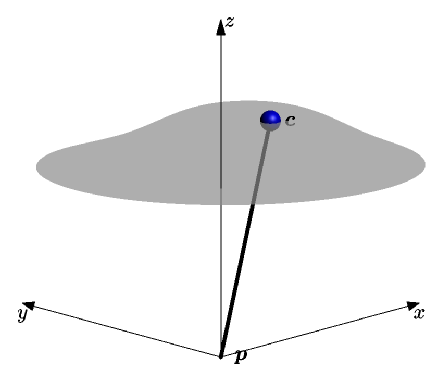
\includegraphics{inverted_pendulum.eps}}
    \caption{Inverted pendulum with a mass $\V{c}$ constrained to a plane.}
    \label{fig.inverted_pendulum}
\end{figure}


\nameref{model.NPM} model is usually linearized with respect to the \ac{CoM}
motion by taking $\C{c}^z$ to be constant and, consequently, $\ddotC{c}^z = 0$
(\cref{ass.fixed_z_coordinate}) \cite{Kajita2003icra}. In addition to this the
following assumptions are commonly made
%
\begin{description}
    \item[\ass{ass.known_ext_wrench}] Wrench $(\forceext,\momentext)$ is known,
        or $\forceextC^z = 0$. This is necessary to linearize the model with
        respect to the external wrench \cite{Agravante2016icra}. In the
        following we assume that $(\forceext,\momentext)$ is a known constant
        for simplicity.

    \item[\ass{ass.linear_convex_hull}] Constraint
        \cref{eq.nonlinear_point_mass.cop_ctr} on the \ac{CoP} positions is
        expressed with a set of linear equality and inequality constraints. The
        conditions under which this is true are discussed in
        \cref{sec.surface_contacts}.

    \item[\ass{ass.sufficient_friction}] Proxy constraints
        \cref{eq.nonlinear_point_mass.proxy} and constraints on the surface
        contact forces
        \cref{eq.nonlinear_point_mass.friction,eq.nonlinear_point_mass.nonzero_z_force}
        are always satisfied. They can, however, be imposed explicitly if
        necessary.
\end{description}
%
Then the model is reduced to
%
\begin{subequations}\label{eq.linear_point_mass}
    \begin{empheq}[left=\empheqlbrace]{align}
        &
            \cop
            =
            \V{c}^{xy}
            -
            \zeta
            \ddotV{c}^{xy}
            +
            \FUNC{Z}(\zeta, \V{g}, \forceext, \momentext)
            ,
            \label{eq.linear_point_mass.cop_eq}
            \\
        &
            \zeta
            =
            \frac{m (c^z - \contactC^z)}{- m \C{g}^z - \forceextC^z}
            ,
            \\[2mm]
        &
            \cop \in \SET{S}(\contact_1^{xy}, ... ,\contact_{M_s}^{xy})
            ,
            \label{eq.linear_point_mass.cop_ctr}
    \end{empheq}
\end{subequations}
%
where the function $\FUNC{Z}(\zeta, \V{g}, \forceext, \momentext)$ represents
the contribution of the external wrench and gravity to the \ac{CoP} position:
%
\begin{equation}
    \FUNC{Z}(\zeta, \V{g}, \forceext, \momentext)
    =
    \zeta
    \left(
        \V{g}^{xy}
        +
        \frac{\forceext^{xy}}{m}
    \right)
    +
    \frac{1}{- m \C{g}^z - \forceextC^z}
    \begin{bmatrix}
        - \momentextC^y\\
        \momentextC^x\\
    \end{bmatrix}
    ,
\end{equation}
%
The model can be further combined with a double or triple integrator to obtain
a second or third order linear model. There is a number of ways to realize such
a combination. For example, the \ac{CoP} position can be
%
\begin{itemize}
    \item an output of second or third order model \cite{Kajita2003icra,
        Herdt2010auro, Agravante2016icra};

    \item a part of the state of a third order model \cite{Kajita2010iros};

    \item the control input of a second order or third order model
        \cite{Sherikov2014humanoids}.
\end{itemize}
%
Furthermore, the differential equation \cref{eq.linear_point_mass.cop_eq} can
be transformed to expose its stable and unstable parts
\cite{Englsberger2011iros, Krause2012src, Takenaka2009iros}, see also
\cref{sec.point_mass_planar_capturability}. Another common approach taken in
the literature consist in collapsing the surface contacts to point contacts,
which greatly simplifies constraint \cref{eq.linear_point_mass.cop_ctr}
\cite{Englsberger2011iros}: if $M_s = 1$ then $\cop = \contact_1^{xy}$, if $M_s
= 2$ then $\cop$ lies on a segment $[\contact_1^{xy}, \contact_2^{xy}]$, \ETC.
The differences between the various versions of the model are often subtle, but
there are certain general considerations to keep in mind while choosing a
particular version:
%
\begin{itemize}
    \item Force sensors in the feet of modern robots allow for the
        determination of the position of the \ac{CoP}
        \cite{Englsberger2014humanoids, Kaneko2004icra, Kaneko2009humanoids},
        which suggests its inclusion into the state of the model.

    \item Third order models imply a smooth variation of \ac{CoM} acceleration
        contrary to second order models. A discontinuous change of \ac{CoM}
        acceleration results in a discontinuous change of the \ac{CoP}
        position, which are difficult to realize for humanoid robots
        \cite{Kajita2010iros}.

    \item Discretization of models controlled with piece-wise constant \ac{CoM}
        acceleration or \tn{jerk} (derivative of acceleration) leads to some
        minor difficulties in the satisfaction of constraint
        \cref{eq.linear_point_mass.cop_ctr}. Moreover, the number of times this
        constraint is imposed can be larger than in other cases and its
        satisfaction is not guaranteed at all times. These issues are discussed
        later in \cref{sec.point_mass_planar_discret_jerk}, where the models
        are discretized to be used in \ac{MPC} schemes.
\end{itemize}
%


In the following we are going to consider two third order models, whose state
includes positions, velocities, and accelerations of the \ac{CoM} in the
$x$-$y$ plane
%
\begin{equation}
    \V{x} =
    (
        \C{c}^x,
        \dotC{c}^x,
        \ddotC{c}^x,
        \C{c}^y,
        \dotC{c}^y,
        \ddotC{c}^y
    ).
\end{equation}
%
The models differ in their control inputs:
%
\begin{enumerate}
    \item The first one is controlled by the third derivative (\tn{jerk}) of
        the \ac{CoM} position~\cite{Kajita2003icra, Herdt2010auro,
        Agravante2016icra}
        %
        \begin{model}{CPPMJ}{Continuous Planar Point-Mass controlled with \acs{CoM} Jerk}
        \begin{subequations}\label{eq.point_mass_jerk_control}
            \begin{empheq}[left=\empheqlbrace]{align}
                &
                    \dotV{x}
                    =
                    \begin{bmatrix}
                        \tildeM{A}  & \M{0} \\
                        \M{0} & \tildeM{A}  \\
                    \end{bmatrix}
                    \V{x}
                    +
                    \begin{bmatrix}
                        \tildeV{B} & \V{0}\\
                        \V{0} & \tildeV{B} \\
                    \end{bmatrix}
                    \dddotV{c}^{xy}
                    ,
                    \\
                &
                    \cop
                    =
                    \begin{bmatrix}
                        \tildeM{D} & \M{0}\\
                        \M{0} & \tildeM{D}\\
                    \end{bmatrix}
                    \V{x}
                    +
                    \FUNC{Z}(\zeta, \V{g}, \forceext, \momentext)
                    ,
                    \label{eq.point_mass_jerk_control.cop}
                    \\[2mm]
                &
                    \cop \in \SET{S}(\contact_1^{xy}, ... ,\contact_{M_s}^{xy})
                    ,
            \end{empheq}
        \end{subequations}
        \end{model}
        %
        where
        %
        \begin{equation}
            \tildeM{A}
            =
            \begin{bmatrix}
                0   &  1    & 0    \\
                0   &  0    & 1    \\
                0   &  0    & 0 \\
            \end{bmatrix},
            \quad
            \tildeV{B}
            =
            \begin{bmatrix}
                0  \\
                0  \\
                1  \\
            \end{bmatrix},
            \quad
            \tildeM{D}
            =
            \begin{bmatrix}
                1 & 0 &  - \zeta
            \end{bmatrix}
            .
        \end{equation}
        %
        We do not use this model in our controllers and present it here due to
        its prevalence in the literature.


    \item The second one is controlled by the \ac{CoP} velocity, which is
        obtained by differentiation of \cref{eq.linear_point_mass.cop_eq} under
        assumption that $(\forceext, \momentext)$ is constant
        \cite{Sherikov2014humanoids}
        %
        \begin{model}{CPPMdZ}{Continuous Planar Point-Mass controlled with $\dot{\cop}$}
        \begin{subequations}\label{eq.point_mass_cop_control}
            \begin{empheq}[left=\empheqlbrace]{align}
                &
                    \dotV{x}
                    =
                    \begin{bmatrix}
                        \tildeM{A}  & \M{0} \\
                        \M{0} & \tildeM{A}  \\
                    \end{bmatrix}
                    \V{x}
                    +
                    \begin{bmatrix}
                        \tildeV{B} & \V{0}\\
                        \V{0} & \tildeV{B} \\
                    \end{bmatrix}
                    \dot{\cop},
                    \\
                &
                    \cop
                    =
                    \begin{bmatrix}
                        \tildeM{D} & \M{0}\\
                        \M{0} & \tildeM{D}\\
                    \end{bmatrix}
                    \V{x}
                    +
                    \FUNC{Z}(\zeta, \V{g}, \forceext, \momentext)
                    ,
                    \\[2mm]
                &
                    \cop \in \SET{S}(\contact_1^{xy}, ... ,\contact_{M_s}^{xy})
                    ,
            \end{empheq}
        \end{subequations}
        \end{model}
        %
        where
        %
        \begin{equation}
            \tildeM{A}
            =
            \begin{bmatrix}
                0   &  1  &   0 \\
                0   &  0  &  1 \\
                0   &  \frac{1}{\zeta}   &  0   \\
            \end{bmatrix},
            \quad
            \tildeV{B}
            =
            \begin{bmatrix}
                0   \\
                0   \\
                -\frac{1}{\zeta}\\
            \end{bmatrix}
            , \quad
            \tildeM{D}
            =
            \begin{bmatrix}
                1 & 0 &  - \zeta
            \end{bmatrix}
            .
        \end{equation}
        %
        Here we assumed that
        %
        \begin{description}
            \item[\ass{ass.nonzero_com_height}] $\zeta \ne 0$ or $c^z -
                \contactC^z \ne 0$, \IE, the \ac{CoM} position is not in
                the same plane as contacts.
        \end{description}
        %
        If \cref{ass.nonzero_com_height} does not hold, \nameref{model.CPPMJ}
        and \nameref{model.CPPMdZ} models become equivalent.
\end{enumerate}
%



%%%%%%%%%%%%%%%%%%%%%%%%%%%%%%%%%%%%%%%%%%%%%%%%%%%%%%%%%%%%%%%%%%%%%%%%%%%%%%%%
\subsection{Linear point-mass model with nonplanar CoM motion}\label{sec.point_mass_nonplanar}

Walking with planar motion of the \ac{CoM} (\cref{ass.fixed_z_coordinate}) is
considered to be unnatural and inefficient in terms of energy. In order to
address these issues we proposed to construct a model, which allows for
vertical motion of the \ac{CoM} \cite{Brasseur2015humanoids}. This is achieved
by making the model robust to the motion of the \ac{CoM} along the $z$ axis.


Let us consider \nameref{model.NPM} model
%
\begin{subequations}
    \begin{empheq}[left=\empheqlbrace]{align}
        &
            \cop
            =
            \V{c}^{xy}
            -
            \zeta
            \left(
                \ddotV{c}^{xy} - \V{g}^{xy}  - \frac{\forceext^{xy}}{m}
            \right)
            +
            \underbrace{
                \frac{1}{m (\ddotC{c}^z - \C{g}^z) - \forceextC^z}
            }_{\zeta / (m c^z)}
            \begin{bmatrix}
                - \momentextC^y \\
                \momentextC^x \\
            \end{bmatrix}
            ,
            \\
        &
            \zeta
            =
            \frac{m c^z}{m (\ddotC{c}^z - \C{g}^z) - \forceextC^z}
            ,
            \\[2mm]
        &
            \cop \in \SET{S}(\contact_1^{xy}, ... ,\contact_{M_s}^{xy})
            ,
    \end{empheq}
\end{subequations}
%
where some of the constraints are omitted for simplicity and the support area
is assumed to be linear with respect to contact points
(\cref{ass.sufficient_friction,ass.linear_convex_hull}). One can observe that
if
%
\begin{description}
    \item[\ass{ass.ext_wrench_zero}] the external wrench is equal to zero
        $(\forceext, \momentext) = \V{0}$,
\end{description}
%
the position of the \ac{CoP} is linear with respect to parameter $\zeta$:
%
\begin{subequations}
    \begin{empheq}[left=\empheqlbrace]{align}
        &
            \cop^{xy}
            =
            \V{c}^{xy}
            -
            \zeta
            (
                \ddotV{c}^{xy} - \V{g}^{xy}
            )
            ,
            \\
        &
            \zeta
            =
            \frac{c^z - \contactC^z}{\ddotC{c}^z - \C{g}^z}
            ,
            \\[2mm]
        &
            \cop \in \SET{S}(\contact_1^{xy}, ... ,\contact_{M_s}^{xy})
            .
    \end{empheq}
\end{subequations}
%
Thus, if $\zeta$ is bounded $\ubar{\zeta} \le \zeta \le \bar{\zeta}$, the
\ac{CoP} position $\cop$ lies on a line segment between two points
$\ubar{\cop}$ and $\bar{\cop}$ as shown in \cref{fig.support_area_zeta}, where
%
\begin{equation}
    \ubar{\cop}
    =
    \V{c}^{xy}
    -
    \ubar{\zeta}
    (\ddotV{c}^{xy} - \V{g}^{xy}),
    \quad
    \bar{\cop}
    =
    \V{c}^{xy}
    -
    \bar{\zeta}
    (\ddotV{c}^{xy} - \V{g}^{xy}).
\end{equation}
%
\begin{figure}[ht]
    \centering{%
    \includegraphics{support_area_zeta.eps}}
    \caption[Robust constraints on the Center of Pressure position.]{
        Grey area represents support area $\SET{S}(\contact_1^{xy},
        \contact_2^{xy})$ of two rectangular foot contacts. The \ac{CoP}
        position lying on a line segment between two points is shown in red.
    }%
    \label{fig.support_area_zeta}%
\end{figure}%
%
At the same time, $\ubar{\cop} \in \SET{S}(\contact_1^{xy}, ... ,
\contact_{M_s}^{xy})$ and $\bar{\cop} \in \SET{S}(\contact_1^{xy}, ... ,
\contact_{M_s}^{xy})$ imply $\cop \in \SET{S}(\contact_1^{xy}, ... ,
\contact_{M_s}^{xy})$ due to convexity of the support area (see
\cref{fig.support_area_zeta}). Hence, we construct a system of linear
constraints on the 3-dimensional motion of the \ac{CoM} as follows
%
\begin{subequations}
    \begin{empheq}[left=\empheqlbrace]{align}
        &
            \ubar{\cop}
            =
            \V{c}^{xy}
            -
            \ubar{\zeta}
            (\ddotV{c}^{xy} - \V{g}^{xy})
            ,
            \\
        &
            \bar{\cop}
            =
            \V{c}^{xy}
            -
            \bar{\zeta}
            (\ddotV{c}^{xy} - \V{g}^{xy}),
            \\
        &
            \ubar{\zeta} (\ddotC{c}^z - \C{g}^z)
            \le
            c^z - \contactC^z
            \le
            \bar{\zeta} (\ddotC{c}^z - \C{g}^z)
            ,
            \\
        &
            \ubar{\cop} \in \SET{S}(\contact_1^{xy}, ... ,\contact_{M_s}^{xy})
            ,
            \\
        &
            \bar{\cop} \in \SET{S}(\contact_1^{xy}, ... ,\contact_{M_s}^{xy})
            ,
    \end{empheq}
\end{subequations}
%
where $\ubar{\zeta}$ and $\bar{\zeta}$ are predefined constants. This system
is then combined with the triple integrator to model motion of the \ac{CoM}
%
\begin{model}{CNPM}{Continuous Nonplanar Point-Mass}
\begin{subequations}
    \begin{empheq}[left=\empheqlbrace]{align}
        &
            \dotV{x}
            =
            \diag{3}{\tildeM{A}}
            \V{x}
            +
            \diag{3}{\tildeM{B}}
            \dddotV{c}
            ,
            \\
        &
            \ubar{\zeta} (\ddotC{c}^z - \C{g}^z)
            \le
            c^z - \contactC^z
            \le
            \bar{\zeta} (\ddotC{c}^z - \C{g}^z)
            ,
            \\[2mm]
        &
            \V{c}^{xy}
            -
            \ubar{\zeta}
            (\ddotV{c}^{xy} - \V{g}^{xy})
            \in
            \SET{S}(\contact_1^{xy}, ... ,\contact_{M_s}^{xy})
            ,\\
        &
            \V{c}^{xy}
            -
            \bar{\zeta}
            (\ddotV{c}^{xy} - \V{g}^{xy})
            \in
            \SET{S}(\contact_1^{xy}, ... ,\contact_{M_s}^{xy})
            ,
            \\[2mm]
        &
            \V{x} =
            (
                \C{c}^x,
                \dotC{c}^x,
                \ddotC{c}^x,
                \enspace
                \C{c}^y,
                \dotC{c}^y,
                \ddotC{c}^y,
                \enspace
                \C{c}^z,
                \dotC{c}^z,
                \ddotC{c}^z
            )
            ,
    \end{empheq}
\end{subequations}
\end{model}
%
where
%
\begin{equation}
    \tildeM{A}
    =
    \begin{bmatrix}
        0   &  1    & 0    \\
        0   &  0    & 1    \\
        0   &  0    & 0 \\
    \end{bmatrix},
    \quad
    \tildeV{B}
    =
    \begin{bmatrix}
        0  \\
        0  \\
        1  \\
    \end{bmatrix}
    .
\end{equation}
%



%%%%%%%%%%%%%%%%%%%%%%%%%%%%%%%%%%%%%%%%%%%%%%%%%%%%%%%%%%%%%%%%%%%%%%%%%%%%%%%%
%%%%%%%%%%%%%%%%%%%%%%%%%%%%%%%%%%%%%%%%%%%%%%%%%%%%%%%%%%%%%%%%%%%%%%%%%%%%%%%%
%%%%%%%%%%%%%%%%%%%%%%%%%%%%%%%%%%%%%%%%%%%%%%%%%%%%%%%%%%%%%%%%%%%%%%%%%%%%%%%%
\section{Limitations of the approximate models}\label{sec.approx_models_limitations}

We conclude our survey of approximate models with a reflection upon their
limitations and the means of relaxing these limitations. In order to do this,
we investigate the assumptions made during the derivation of these models:
%
\begin{itemize}
    \item We abstract from the complex structure of the robot's body
        (\cref{ass.nojointctr}). Hence, we lose the ability to express some of
        the whole body tasks and constraints. For example, the point-mass model
        does not allow to specify a reaching task for a hand. Therefore, when
        it is necessary to bias motion previewed with this model by a hand
        task, it is common to resort to various \emph{ad hoc} approaches
        \cite{Yoshida2006humanoids, Nishiwaki2003icra, Fukumoto2004iros}. Whole
        body constraints are often approximated by proxy constraints
        (\cref{sec.nonlinear_approx_models}). For example, the position of the
        \ac{CoM} is limited with respect to foot positions in
        \cite{Brasseur2015humanoids, Dellin2012icra} to avoid kinematic
        infeasibility. Another general approach to take into account whole body
        tasks and constraints is to employ \ac*{MMPC}, which was proposed in
        \cite{Sherikov2014humanoids} and is described in \cref{sec.mmpc}.


    \item We presume that the rate of angular momentum is zero in the
        point-mass model (\cref{ass.point_mass}) or takes arbitrary values in
        the momenta based model (\cref{sec.model_momenta}). Neither of this is
        true in reality: execution of limb motions implies certain values of
        rate of angular momentum. These values can be estimated using
        multi-mass models, some of which are linear
        \cite[Chapter~3]{Herdt2012thesis}, \cite{Lafaye2014humanoids,
        Shimmyo2013tie, Takenaka2009iros}.


    \item Bilinearity of the rate of angular momentum with respect to the
        \ac{CoM} motion and contact forces as follows from Equation
        \cref{eq.newton-euler} is addressed with two assumptions:
        %
        \begin{itemize}
            \item The angular momentum about the $z$ axis is typically
                disregarded
                (\cref{ass.arbitrary_z_momentum,ass.arbitrary_z_moment}).
                Significance of implications of this is currently unclear to
                us.

            \item Motion of the \ac{CoM} is fixed to a plane
                (\cref{ass.fixed_z_coordinate}). There exists a number of
                approaches to cope with this \cite{Nishiwaki2011icra,
                Feng2013humanoids}, in particular, we proposed to introduce
                robustness with respect to nonplanar \ac{CoM} motion
                \cite{Brasseur2015humanoids}, \cref{sec.point_mass_nonplanar}.
        \end{itemize}

        %
        \begin{equation}\label{eq.newton-euler}
            \begin{bmatrix}
                \dotV[c]{\LM} \\
                \dotV[c]{\AM}\\
            \end{bmatrix}
            =
            \begin{bmatrix}
                m\V{g}\\
                \V{0}
            \end{bmatrix}
            +
            \sum_{i=1}^M
                \begin{bmatrix}
                    \M{I}                     & \M{0}\\
                    \CROSS[(\contact_i - \V{c})]   & \M{I}
                \end{bmatrix}
                \begin{bmatrix}
                    \force_i\\
                    \M[i]{R} \moment[i]_i
                \end{bmatrix}.
        \end{equation}
        %

    \item Bilinearity of the rate of angular momentum with respect to the
        contact positions and contact forces as follows from Equation
        \cref{eq.newton-euler} is dealt with by predetermining either contact
        positions or magnitudes of the contact forces. For example, we fix
        contact positions in the momenta based model (\cref{ass.fixed_points}).
        On the other hand, in the case of a single contact, when the force is
        determined by the \ac{CoM} motion, the contact position may vary (see
        \cite{Herdt2010auro} and \cref{sec.surface_contacts}). When it is
        undesirable to predetermine contact positions and forces, it is common
        to employ nonlinear models \cite{Dai2014humanoids, Tassa2014icra}.
\end{itemize}
%

It is important to note that some of these limitations can be lifted in
discrete-time models, since such models allow for different parameters on
different discretization intervals. For example, in discrete-time the number
and positions of contacts in the momenta-based model may vary, as well as the
height of the contact surface $\contactC^z$ in the point-mass model with
nonplanar \ac{CoM} motion. This topic is discussed in more detail in
\cref{sec.discret_variation}.



%%%%%%%%%%%%%%%%%%%%%%%%%%%%%%%%%%%%%%%%%%%%%%%%%%%%%%%%%%%%%%%%%%%%%%%%%%%%%%%%
%%%%%%%%%%%%%%%%%%%%%%%%%%%%%%%%%%%%%%%%%%%%%%%%%%%%%%%%%%%%%%%%%%%%%%%%%%%%%%%%
%%%%%%%%%%%%%%%%%%%%%%%%%%%%%%%%%%%%%%%%%%%%%%%%%%%%%%%%%%%%%%%%%%%%%%%%%%%%%%%%
\section{Conclusion}

This chapter serves as a survey of the whole body model of a humanoid robot and
approximate models derived from it. The models are presented in a unified view,
which is not very common in the literature, where the focus is typically made
on particular models and applications. The author's contribution to the subject
consists in a participation to collaborative works which employ approximate
models \cite{Agravante2016icra, Brasseur2015humanoids}.
